%% entwurf.tex
%% $Id: entwurf.tex 28 2007-01-18 16:31:32Z bless $
%%
%% ==============================
\chapter{Konzeption}
\label{ch:Design}
In diesem Kapitel werden die Anforderungen an die Forscherplattform und den hierfür benötigten Therapiemodellierungsansatz beleuchtet. Für diese werden zunächst die Persona dargestellt. Diese beschreiben verschiedene Eigenschaften der Personengruppen, die später den \emph{TherapyBuilder} bedienen, der in Kapitel \ref{ch:Background}  beschriebenen wird. Anschließend werden verschiedene Studien betrachtet, die von Psychologen entwickelt wurden. Die Studien bestehen aus Therapien, die beispielsweise auf ihre Wirksamkeit geprüft werden. Aus den Defiziten der Technologien, die im Stand der Technik diskutiert werden, den dargestellten Persona und den Studieneingenschaften, werden die Anforderungen an den Therapiemodellierungsansatz entwickelt. Auf Basis der Anforderungsanalyse werden verschiedene Konzepte entwickelt. Hierfür werden zunächst wichtige Begriffe und Strukturen definiert, die für das Verständnis der Konzepte relevant sind.


\section{Anforderungsanalyse}
Nachfolgend werden die verschiedenen Aspekte beleuchtet, die für eine Anforderungsanalyse relevant sind. Basierend auf diesen Aspekten werden die Anforderungen formuliert.

\subsection{Persona}
Die in Kapitel \ref{ch:Background} beschriebene \emph{TherapyBuilder}-Plattform wird voraussichtlich von drei Personengruppen verwendet. Der Forscher bedient die Forscher-Plattform. Auf dieser werden die Chatbots und deren Steuerung entwickelt. Durch die Therapeuten-Plattform haben Forscher und Therapeuten die Möglichkeit die Patienten oder Studienteilnehmer zu verwalten und diesen verschiedene Therapien zuzuordnen. Die App hingegen wird hauptsächlich von Patienten benutzt. Diese können allerdings auch Studienteilnehmer sein. Die Rollen werden in diesem Kapitel genauer beschrieben.

\subsubsection{Forscher}
Der Forscher entwickelt neue Therapien. Diese werden in Studien auf ihre Wirksamkeit getestet. Betrachtet werden das Profil und die Ziele des fiktiven Forscher \emph{Prof. Dr. Richard Weimer}. 

\begin{figure}[h]
\centering

\includegraphics[width=1\textwidth]{pictures/forscher}
\caption{Eckdaten des fiktiven Forschers \emph{Prof. Dr. Richard Weimer}}
\label{forscher}
\end{figure}

\paragraph{Profil} 
\emph{Prof. Dr. Richard Weimer} ist Psychologe. Er leitet die Abteilung für Persönlichkeitsforschung eines Psychologischen Instituts einer Universität. Er lebt in Heidelberg nahe der Universität. Sein Interesse gilt der Entwicklung und Verbesserung von Therapien für Angststörungen. Neben der Lehre erarbeitet er zusammen mit Studenten und wissenschaftlichen Mitarbeitern neue Therapie-Konzepte. Diese werden auf ihre Wirksamkeit überprüft. Die Ergebnisse werden in Form einer wissenschaftlichen Arbeit publiziert.

Er nutzt seine Freizeit gerne um sich über neue Therapie-Methoden zu informieren und neue Technologien zu erschließen die Therapien verbessern können. Meist hält er Notizen und neue Therapiekonzepte auf Papier fest. Für Studien werden diese in Excel-Tabellen eingepflegt. Die Auswertungen macht er bislang teils manuell, teils automatisiert über Excel.

Zusammen mit Studenten und wissenschaftlichen Mitarbeitern entwickelt er Anwendungen für Probanden die begleitend zur Therapie eingesetzt werden. Mit ihnen sucht er auch nach neuen Möglichkeiten Therapien mit wenig Papier übersichtlich zu gestalten und Daten schneller gesammelt und anonymisiert auszuwerten. Dabei sollen Studiendesign wie Ergebnisse nachvollziehbar für wissenschaftliche Arbeiten dokumentiert werden.


\paragraph{Ziele}
\begin{itemize}
\item Übersichtliche Studien-Dokumentation
\item Einfache und gesammelte Datenauswertung
\item Übersichtliches Erstellen einer Therapie
\item Nutzung neuer Technologien für Therapien
\item Nutzung verschiedener Plattformen für Therapie 
\end{itemize}


\subsubsection{Therapeut}
Der Therapeut wendet Therapien auf Patienten an. Basierend auf den Patientenprofilen ordnet er diesen verschiedene Therapien zu. Betrachtet werden das Profil und die Ziele der fiktiven Therapeutin \emph{Dipl.-Psych. Barbara Probst}

\begin{figure}[h]
\centering
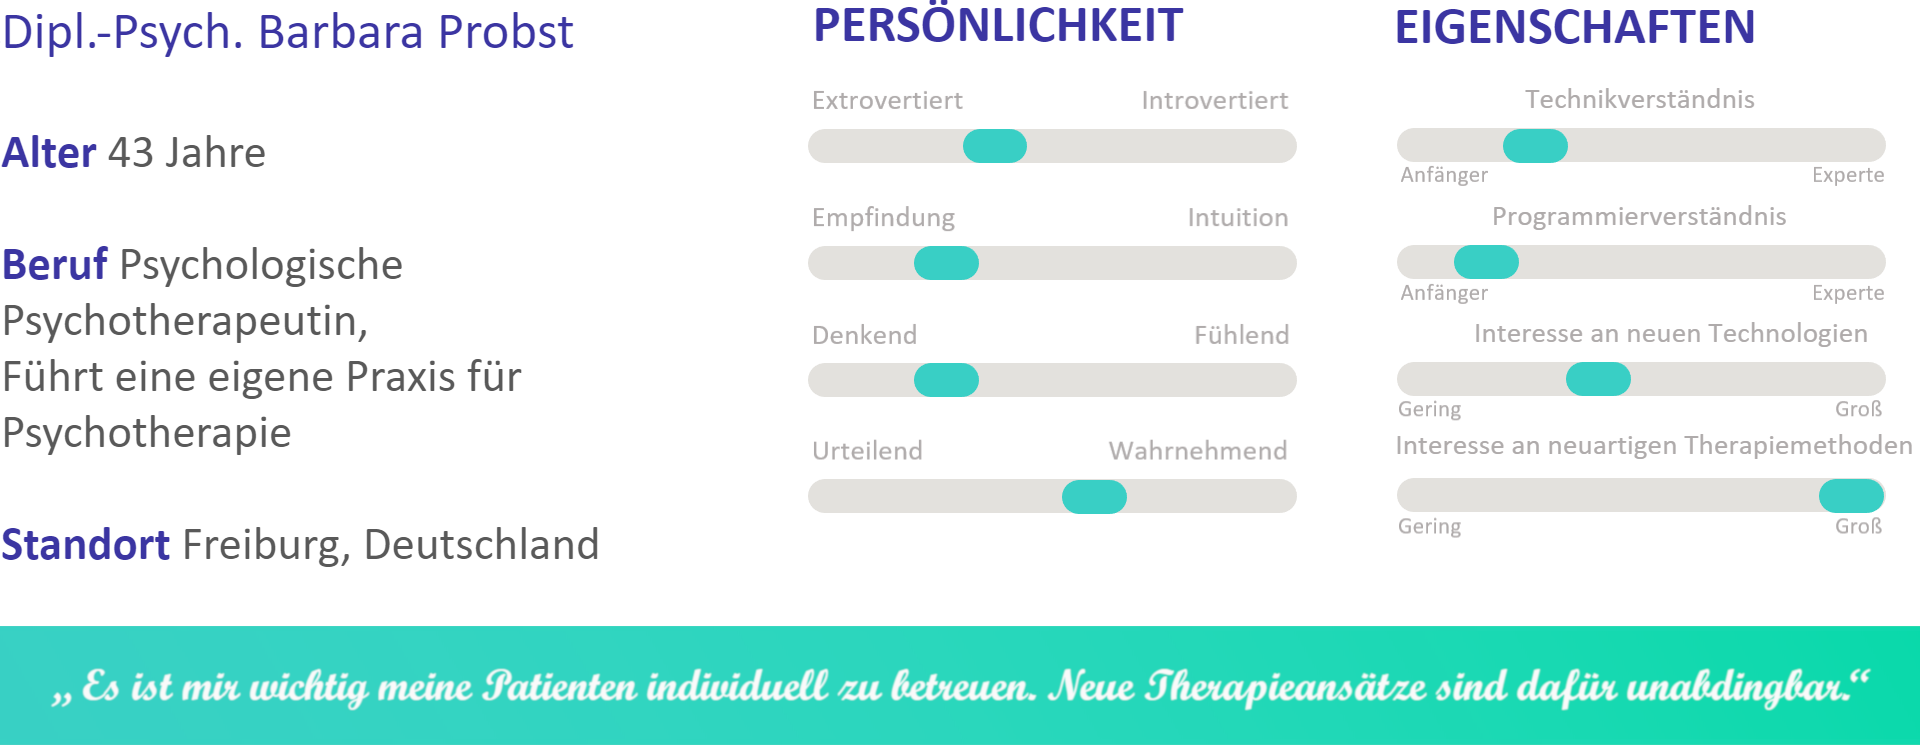
\includegraphics[width=1\textwidth]{pictures/therapeut}
\caption{Eckdaten der fiktiven Therapeutin \emph{Dipl.-Psych. Barbara Probst}}
\label{therapeut}
\end{figure}

\paragraph{Profil}
\emph{Dipl.-Psych. Barbara Probst} ist staatlich geprüfte psychologische Psychotherapeutin. Sie führt eine eigene Praxis. In dieser behandelt sie Patienten mit verschiedenen Störungen mit Krankheitswert. Ihr Spezialgebiet ist die Angststörung.

Sie wendet verschiedene Therapieansätze an. Diese werden individuell auf Persönlichkeit, Krankheitsverlauf und Symptomen des Patienten ausgewählt und zugeschnitten. Dabei nutzt sie altbewährte, wie auch neue Therapieansätze. Ihr Interesse gilt insbesondere neuartigen Therapiemethoden im Bereich der Angststörung. In ihrer Freizeit beschäftigt sie sich deshalb mit Fachjournalen. Sobald sie eine neue vielversprechende und geprüfte Therapiemethode entdeckt, notiert sie sich verschiedene Ansätze um diese auf geeignete Patienten zu übertragen. Dabei sind besonders Ansätze interessant, die neuartige Technologien verwenden.

Da ihr Stundenplan voll belegt ist muss die Übertragung neuer Therapiemethoden leicht und schnell gehen. Falls neue Technologien notwendig sind, sollen diese so leicht zu bedienen sein, dass kein Mehraufwand in Dokumentation und Planung entsteht. Außerdem ist es wichtig, dass eingesetzte Technologien wenig Aufwand und Expertenwissen benötigen um diese entsprechend einzurichten und zu bedienen.

\paragraph{Ziele}
\begin{itemize}
\item Austesten neuer Therapiemethoden
\item Einsatz neuer Technologien in Verbindung mit Psychotherapie
\item Neue Technologien sollten keinen Mehraufwand an Dokumentation darstellen
\item Neue Technologien und Therapien sollten keinen Mehraufwand an Planung darstellen
\item Einsatz neuer Therapiemethoden trotz wenig Zeit
\item Leicht integrierbar in den Alltag und das System eines Psychotherapeuten
\item Geringe Kosten in der Anwendung
\end{itemize}

\subsubsection{Patient}
Der Patient nutzt auf seinem Smartphone die \emph{TherapyBuilder}-App. Diese führt die Therapien aus, die dem Patienten vom Therapeut zugeordnet wurde. Betrachtet werden das Profil und die Ziele der fiktiven Patienten \emph{Jonas Vogt}.

\begin{figure}[h]
\centering
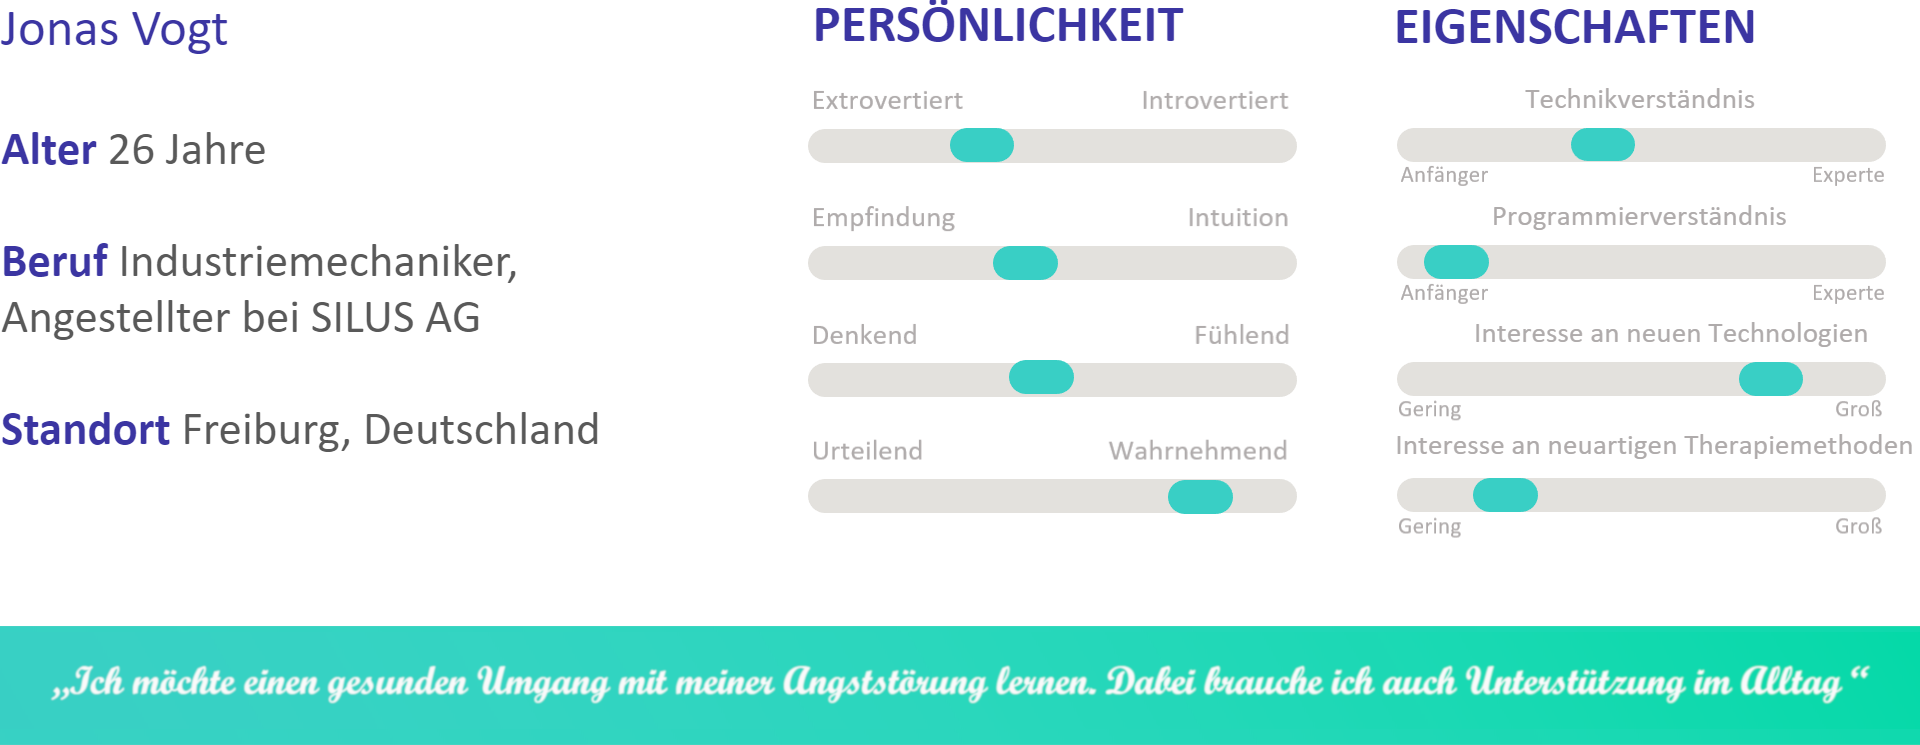
\includegraphics[width=1\textwidth]{pictures/patient}
\caption{Eckdaten des fiktiven Patienten \emph{Jonas Vogt}}
\label{patient}
\end{figure}

\paragraph{Profil}
\emph{Jonas} ist Industriemechaniker aus Freiburg. Er ist seit 3 Jahren Angestellter bei SILUS AG. Nach einem Jahr wurde er zum Schichtleiter befördert. Die Arbeit macht ihm sehr viel Freude. Er ist pflichtbewusst und nimmt seine Verantwortung als Schichtleitung ernst. Er beschäftigt sich in seiner Freizeit fast täglich mit neuen Strategien und Techniken für einen effizienten Schichtbetrieb. Aufgrund seines fachlichen Wissens und Engagements tauschen sich Arbeitskollegen wie Chefs gerne über neue Strategien mit ihm aus.

Neben seinem Beruf interessiert er sich für neue Technik-Gadgets, Spielekonsolen und Multimedia. In seiner Freizeit trifft er sich gerne mit Freunden zum Feiern, gemeinsamen Kochen aber auch zu gemütlichen Film und Spieleabenden. Er verabredet sich häufig über diverse Messenger und teilt über diese gerne Artikel über neue Technik-Gadgets.

\emph{Jonas} hat eine Angststörung die als Begleiterscheinung eines Burn-outs während der Ausbildung auftrat.  Derzeit wartet er auf seine erste Therapiesitzung bei \emph{Dipl.-Psych. Barbara Probst}. Während der Wartezeit nutzt er einen Chatbot. Diesen setzt er ein sobald er sich unwohl fühlt und die Angststörung auftritt. Seine Psychotherapeutin empfahl \emph{Jonas} diesen Chatbot während der Wartezeit zu nutzen.

\paragraph{Ziele}
\begin{itemize}
\item Behandeln der Angststörung
\item Hilfe im Alltag wenn Angststörung auftritt
\item Einfache Anwendung der Hilfe
\item Hilfe jederzeit erreichbar
\item Hilfe leicht in Alltag integrierbar
\end{itemize}


\subsection{Studienbetrachtung}
Für die Anforderungsanalyse werden mehrere Studien betrachtet. Diese liegen der Firma \emph{movisens GmbH} in unterschiedlichen Formaten vor. Ablauf und Inhalte der jeweiligen Studie wurden in PowerPoint-Folien, Excel und Bildern, wie beispielsweise in Abbildung \ref{studie}, beschrieben. Jede Studie besitzt Inhalte, die in Form eines Chats umgesetzt werden könnten. Die Studien beinhalten Therapien, die in dieser evaluiert werden. Die Therapien setzen sich aus verschiedenen Stilmitteln zusammen. So finden sich Dialoge die aus Input und Output-Formaten bestehen. Die Input-Formate repräsentieren Formate, die dem Patienten angeboten werden um Daten einzugeben. Die Output-Formate beinhalten Formate, die dem Patienten angezeigt werden. Die Therapien bestehen aus Übungen, Interventionen und Selbstüberwachung.

\begin{figure}[h]
\centering
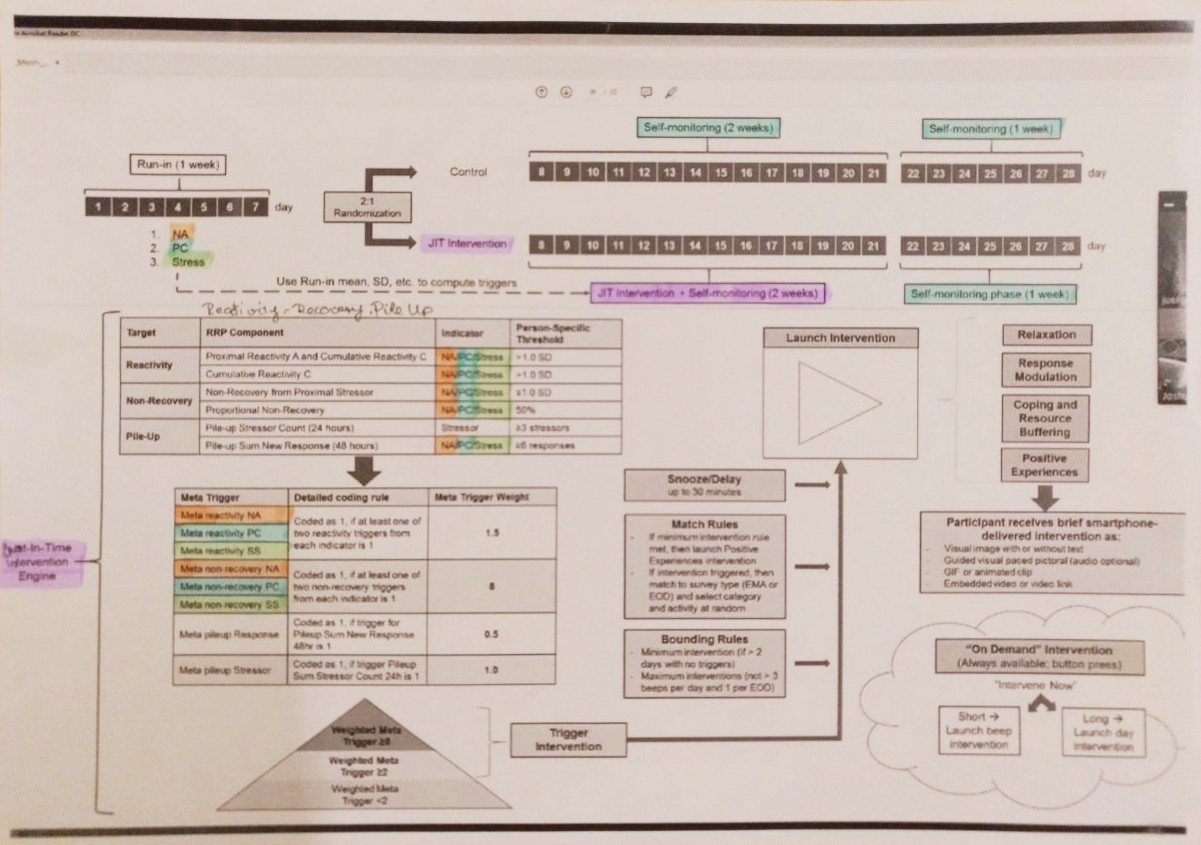
\includegraphics[width=1\textwidth]{pictures/studie}
\caption{Eckdaten des fiktiven Forschers \emph{Prof. Dr. Richard Weimer}}
\label{studie}
\end{figure}

Um eine Therapie umzusetzen, werden als Output-Formate Textausgaben, Video, Audio, und Bilder benötigt. Als Input-Formate für den Patienten werden Texteingabe, ganze Zahlen, rationale Zahlen, Likert-Skalen, visuelle Analogskalen, Einfach- wie Mehrfachauswahl, Zeiteingabe und eine Datumseingabe benötigt. 
 
Da auch Daten erhoben werden, benötigt es Variablen. In diesen werden Antworten und berechnete Werte gespeichert. Die Werte der Variablen können dem Patienten im Text präsentiert werden aber auch den Verlauf der Therapie beeinflussen. So können dem Patienten beispielsweise verschiedene Texte, Übungen oder Interventionen präsentiert werden. Die entsprechenden Inhalte werden zu unterschiedlichen Zeiten und Bedingungen ausgelöst. Auslöser können ein erreichtes Datum, vorgegebene Zeit, Therapeut, Patient oder verschiedene Bedingungen sein. Um diese Übersicht zu erhalten, wurde der zeitliche Ablauf der betrachteten Studien in einem Zeitstrahl abgebildet. Diese zeitliche Skizzierung wird in Abbildung \ref{studien} dargestellt.

\begin{figure}[h]
\centering
\includegraphics[width=1\textwidth]{pictures/studien}
\caption{Die zeitliche Abbildung verschiedener Studien in Form eines Zeitstrahls}
\label{studien}
\end{figure}

\subsection{Defizite der betrachteten Technologien}
In Kapitel \ref{ch:Forschungsstand} werden verschiedene Technologien vorgestellt, die für eine Umsetzung eines \emph{TMA} in Frage kommen. Die dort erläuterten Defizite werden hier in Kurzform zusammengefasst.

\subsubsection{Grafische Programmiersprachen}
Betrachtet wurden Chatbot-Plattformen und allgemeine grafische Programmiersprachen. Chatbot-Plattformen fokussieren sich zumeist auf Marketing, Vertrieb und Support. Die Umsetzung von Studien, die für die Anforderungsanalyse betrachtet wurden, gestaltet sich in diesen Plattformen schwierig. Diese lassen entsprechende Elemente, wie Likert-Skalen, visuelle Analogskalen und eine Patientenverwaltung vermissen. Konversationen als Baum oder Diagramm darzustellen, ist zwar leicht verständlich, allerdings werden diese schnell unübersichtlich wenn mehrere bedingte Pfade eingesetzt werden und die Komplexität der Konversation steigt. Die Gesamtansicht der Konversationen wird demnach auch schwer lesbar. Entweder müssen Verläufe durch scrollen und durchhangeln nachvollzogen werden oder diese werden durch die eingebaute Zoom-Funktion schlechter erkennbar und auffindbar. Manche Plattformen bieten zusätzlich die Möglichkeit, fehlende Funktionen zu implementieren. Die benötigt allerdings Programmiererfahrung. Generell sind bei der Verwendung dieser Plattformen, für eine Umsetzung entsprechender Therapien, mit Einschränkungen oder größeren Einarbeitungszeiten zu rechnen.

Die allgemeinen Programmiersprachen hingegen spezialisieren sich stark auf bestimmte Domänen. Das Baukastenprinzip gewährleistet zwar viel Flexibilität und ist leicht verständlich in der Bedienung, allerdings wird bei steigender Komplexität das entwickelte System leicht unübersichtlich und schwer nachvollziehbar.

\subsubsection{Auszeichnungssprachen}
Die Verwendung von Auszeichnungssprachen bieten visuell zwar eine Trennung aber keine klare Übersicht über den Verlauf einer Konversation. Es benötigt Konzepte um zeitliche Abfolgen einer Therapie, Verzweigungen und Bedingungen zu realisieren und klar darzustellen. Hinzu kommt, dass die Syntax erlernt werden muss. Außerdem benötigt es einen aufwändigen Syntaxcheck um die Fehlersuche in angelegten Chatbot-Konversationen zu erleichtern.   

\subsubsection{Experience Sampling}
Insbesondere das \emph{movisensXS}-System liefert bereits viele Funktionen, die zur Umsetzung der betrachteten Therapien benötigt werden. Allerdings wurde das System für die Fragebogenentwicklung erstellt und müsste entsprechend angepasst werden um dem Chatbot-Format zu entsprechen.  


\subsection{Anforderungen}
Auf Basis der aufgestellten Persona, Betrachtung der Studien und der Defizite der betrachteten Technologien, wurden funktionale sowie nicht-funktionale Anforderungen aufgestellt, die der Therapiemodellierungsansatz erfüllen sollte. Es wurden mehrere Anforderungen in einem Excel-File beschrieben (vgl. \ref{anforderungen}) und entsprechend priorisiert. In diesem Kapitel werden die Anforderungen mit der höchsten Priorität dargestellt. Hierbei handelt es sich um Anforderungen, die den Therapiemodellierungsansatz grundlegend charakterisieren.

\begin{figure}[h]
\centering
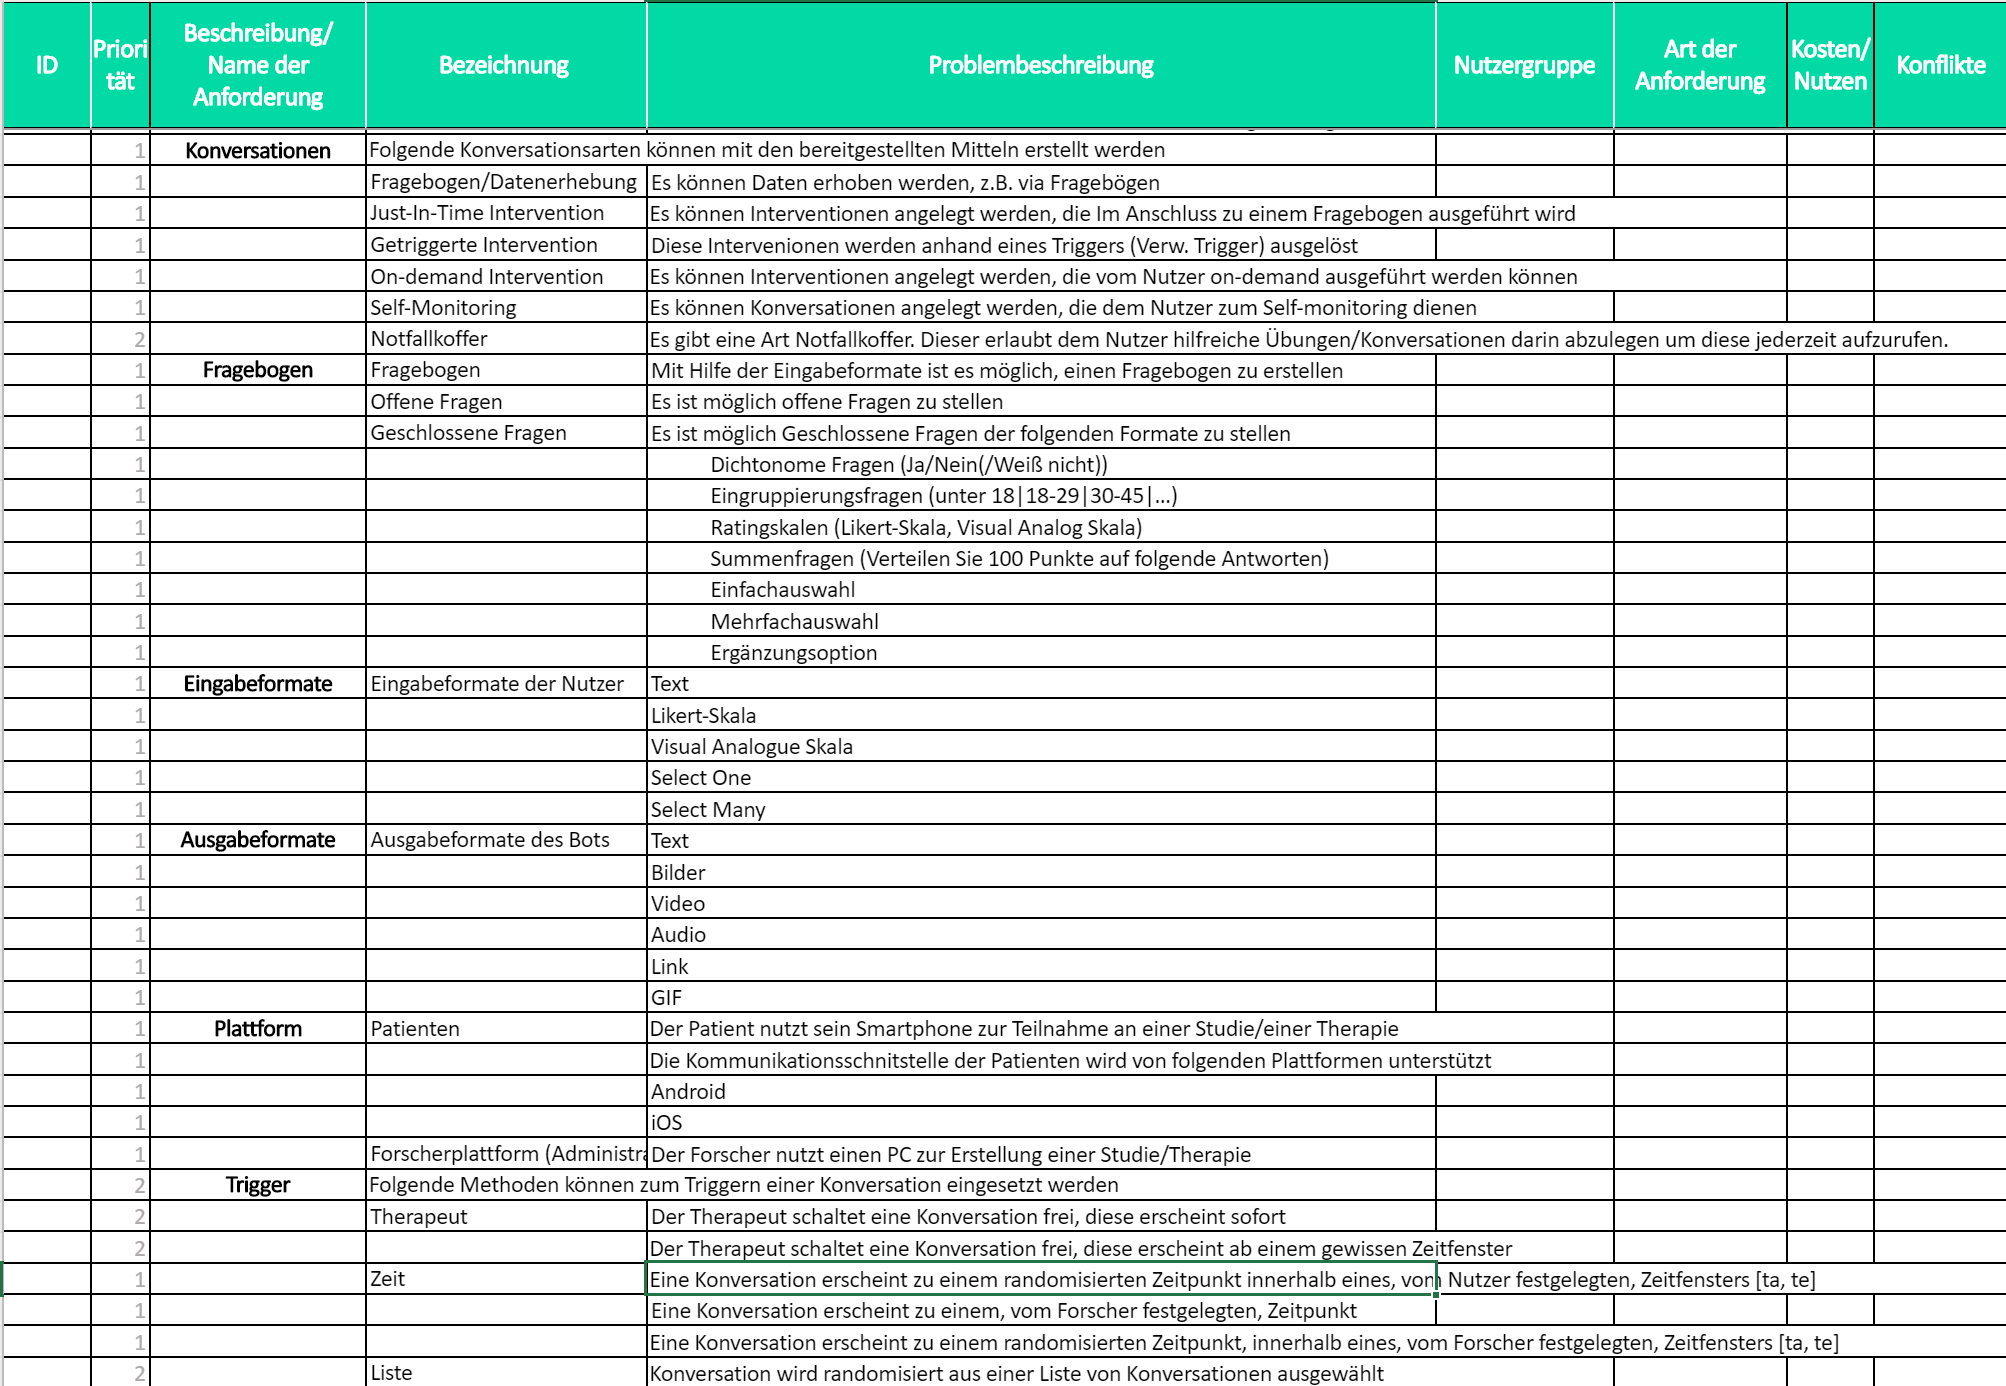
\includegraphics[width=1\textwidth]{pictures/anforderungen}
\caption{Ausschnitt der erstellten Anforderungsliste}
\label{anforderungen}
\end{figure}

\subsection{Funktionale Anforderungen}
Im Folgenden werden die Anforderungen beschrieben, die der Zweckbestimmung der Forscher-Plattform dienen.

\subsubsection{Konversationen}
Folgende Konversationsarten können mit den bereitgestellten Mitteln erstellt werden.

\paragraph{Fragebogen/Datenerhebung} Es können Daten erhoben werden, z.B. via Fragebögen

\paragraph{Just-In-Time Intervention} Es können Interventionen angelegt werden, die im Anschluss zu einem Fragebogen ausgeführt werden.

\paragraph{Getriggerte Intervention} Interventionen werden anhand eines Triggers  ausgelöst.

\paragraph{On-demand Intervention} Es können Interventionen angelegt werden, die vom Nutzer on-demand ausgeführt werden können.

\paragraph{Self-Monitoring} Es können Konversationen angelegt werden, die dem Nutzer zum Self-monitoring dienen.

\subsubsection{Fragebogen}
Mit Hilfe der Eingabeformate ist es möglich, einen Fragebogen zu erstellen. Mit diesen Mitteln können in den Fragebögen verschiedene Frageformen umgesetzt werden.

\paragraph{Offene Fragen} Es ist möglich offene Fragen zu stellen.

\paragraph{Geschlossene Fragen} Es ist möglich Geschlossene Fragen der folgenden Formate zu stellen:

\begin{itemize}
\item Dichtonome Fragen (Ja/Nein(/Weiß nicht))
\item Eingruppierungsfragen (unter 18|18-29|30-45|…)
\item Ratingskalen (Likert-Skala, Visual Analog Skala)
\item Summenfragen (Verteilen Sie 100 Punkte auf folgende Antworten)
\item Einfachauswahl
\item Mehrfachauswahl
\item Ergänzungsoption
\end{itemize}

\subsubsection{Eingabeformate} Eingabeformate der Nutzer	
\paragraph{Freie Texteingabe}
\paragraph{Likert-Skala}
\paragraph{Visual Analogue Skala}
\paragraph{Select One}
\paragraph{Select Many}

\subsubsection{Ausgabeformate} Ausgabeformate des Bots
\paragraph{Text}
\paragraph{Bilder}
\paragraph{Video}
\paragraph{Audio}
\paragraph{Link}
\paragraph{GIF}

\subsubsection{Trigger}Folgende Methoden können zum Triggern einer Konversation eingesetzt werden

\paragraph{Therapeut}Der Therapeut schaltet eine Konversation frei, diese erscheint sofort. 
Der Therapeut schaltet eine Konversation frei, diese erscheint ab einem gewissen Zeitfenster.

\paragraph{Zeit}Eine Konversation erscheint zu einem randomisierten Zeitpunkt innerhalb eines, vom Nutzer festgelegten, Zeitfensters [ta, te].
Eine Konversation erscheint zu einem, vom Forscher festgelegten, Zeitpunkt.
Eine Konversation erscheint zu einem randomisierten Zeitpunkt, innerhalb eines, vom Forscher festgelegten, Zeitfensters [ta, te]

\paragraph{Liste}Konversation wird randomisiert aus einer Liste von Konversationen ausgewählt

\paragraph{Ausführungsanzahl}Eine Konversation kann anhand einer Anzahl Ausführungen an einem Tag getriggert werden

\paragraph{Nutzer}Ein Nutzer kann selbst eine Konversation starten 

\paragraph{Konversation}Eine Konversation kann durch das Abschließen einer anderen Konversation getriggert werden

\paragraph{Snooze}Eine Konversation wird erneut getriggert nach Zeitpunkt des Snoozes eines Nutzers +t (zB. 30 Minuten)

\paragraph{Variable}Eine Konversation wird durch einen Wert einer Variable getriggert
die Variable hat den aktuellen Wert x.
die Variable hatte den Wert x zum Zeitpunkt t.
die Variable wird ermittelt aus verschiedenen Variablen/Werten durch eine vorgegebene Funktion und erfüllt eine Bedingung.

\subsubsection{Variablen}
\paragraph{Speichern}Es können Werte unter Variablennamen abgespeichert werden
\paragraph{Historie}Die Werte, die eine Variable im Verlauf eines Therapiemoduls angenommen hat, werden in einer Historie hinterlegt
\paragraph{Typen} Eine Variable kann einen der folgenden Typen annehmen
\begin{itemize}
\item String
\item Gleitkommazahl
\item Ganze Zahl 
\item Boolean (Wahr/Falsch)
\item Image (DB-Blob)
\item Video (DB-Blob)
\item Audio (DB-Blob)
\item Link
\end{itemize}	

\subsubsection{Flexible Gestaltung von Triggern}

\subsubsection{Verzweigungen in Konversationen}

\subsubsection{Abhängigkeiten zwischen Konversationen}


\subsection{Nicht-Funktionale Anforderungen}
Im Folgenden werden die Anforderungen beschrieben, die der Qualität der Forscher-Plattform dienen.

\paragraph{Anmeldeseite} Nachdem der Nutzer den Link zur TherapyBuilder Forscher-\paragraph{Plattform} in einer Browser Adressleiste eingegeben hat, öffnet sich die Anmeldeseite.

\paragraph{Startseite}Nach erfolgreicher Anmeldung des Nutzers, wird dieser auf die Startseite weitergeleitet
\paragraph{Startseite-Inhalt}Die Startseite beinhaltet
\begin{itemize}
\item Logout: Es gibt ein Link zum Ausloggen
\item Account-Einstellungen: Es gibt ein Link zum Aufrufen der Account-Einstellungen
\item Übersicht bereits angelegter Therapie-Module: Es gibt eine Übersicht über alle bereits angelegte Therapie-Module
\item Therapie-Modul hinzufügen: Es gibt eine Schaltfläche zum Hinzufügen eines Therapie-Moduls
\item Therapie-Modul umbenennen:	Es gibt eine Schaltfläche zum Umbenennen eines Therapie-Moduls
\item Therapie-Modul entfernen:	Es gibt eine Schaltfläche zum Entfernen eines Therapie-Moduls
\item  Therapie-Modul kopieren:	Es gibt eine Schaltfläche zum Kopieren eines Therapie-Moduls
\item Therapie-Modul Status: Jedes bereits angelegte Therapie-Modul erhält einen Status. Dieser Status wird auf der Übersichtsseite für jedes Therapie-Modul angezeigt.
\end{itemize}
	
\paragraph{Bearbeiten} Therapiemodul bearbeiten	Durch Klick auf ein Therapie-Modul, gelangt man auf dessen Bearbeitungsseite
		
\paragraph{Hinzufügen}Durch Klick auf die "Hinzufügen" Schaltfläche wird ein neues Therapie-Modul angelegt.

\paragraph{Umbenennen} Durch Klick auf die "Umbenennen" Schaltfläche kann der Nutzer das Modul umbennenen.

\paragraph{Kopieren} Durch Klick auf die "Kopieren" Schaltfläche kann der Nutzer das Modul kopieren.

\paragraph{Entfernen} Durch Klick auf die "Entfernen" Schaltfläche öffnet sich ein Dialog zur Eingabe des Wortes "DELETE" um das Entfernen des Therapie-Moduls zu bestätigen.


\section{Ausarbeitung verschiedener Konzepte}

\subsection{Begriffsdefinitionen}
Im Rahmen der Konzeption werden verschiedene Begriffe eingeführt, die Klarheit über Struktur und Aufbau einer Therapie geben werden. Unterschieden wird zwischen den Begriffen \emph{Therapie}, \emph{Therapiemodul}, \emph{Chatbot-Konversation}, \emph{Chatbot-Nachricht}, \emph{Werkzeugkasten}. Für ein besseres Verständnis der Zusammenhänge werden Mengendefinitionen abgebildet. Für diese werden die Kürzel aus Abbildung \ref{begriffe} verwendet.


\begin{figure}[h]
	\centering
	\includegraphics[width=.75\textwidth]{pictures/begriffe}
	\caption{Die verwendeten Begriffe und ihre Synonyme.}
	\label{begriffe}
\end{figure}

Insgesamt bestehen zwischen den Begrifflichkeiten Beziehungen die den Aufbau einer Therapie beschreiben. Abbildung \ref{mengeninsg} verdeutlicht den gesamten Aufbau einer Therapie und die Zusammenhänge zwischen einzelnen Elementen. Eine Therapie besteht aus verschiedenen Therapie-Modulen. Diese bilden sich wiederum aus Chatbot-Konversationen. Chatbot-Konversationen können sich aus einfachen Nachrichten zusammenbauen. Es gibt auch Elemente, die in einem Werkzeugkasten als Konversation auftauchen können. Diese können wiederum ein Teil einer Konversation sein und setzen sich ebenfalls aus einfachen Nachrichten zusammen. Die Nachrichten entweder aus Chatbot-Nachrichten oder Patienten-Nachrichten. Die genauen Begrifflichkeiten werden in diesem Kapitel definiert, erklärt und mit Beispielszenarien anhand der entwickelten Persona beschrieben.

\begin{figure}[h]
	\centering
	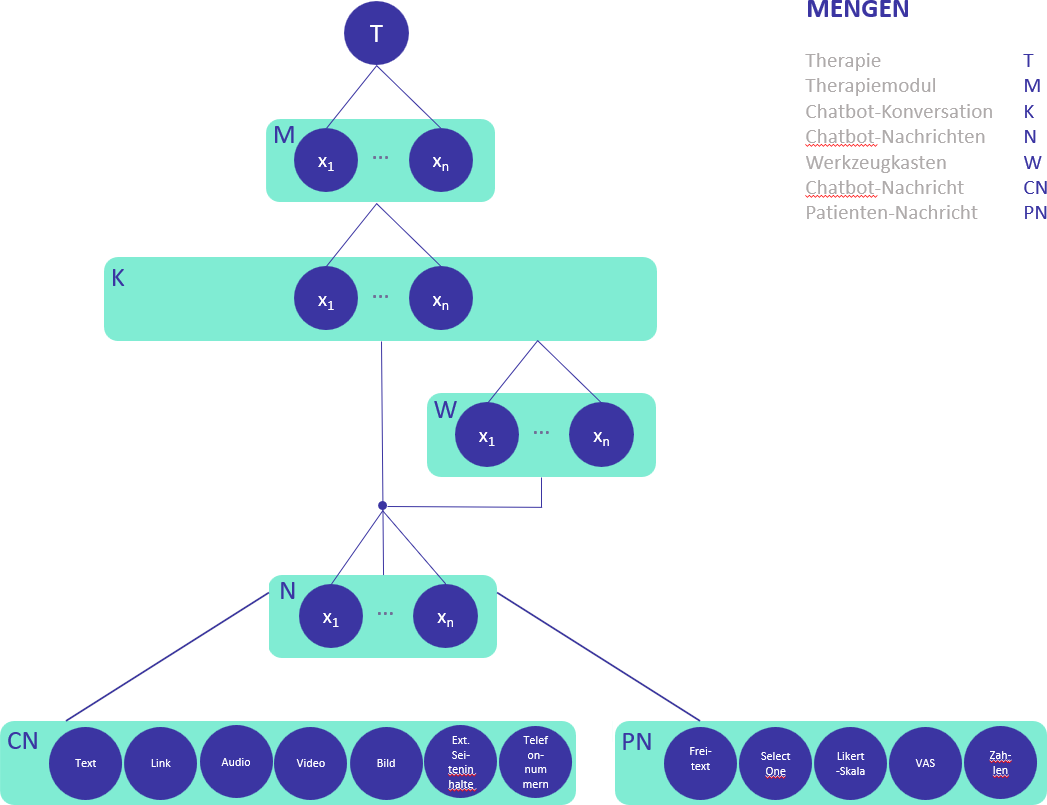
\includegraphics[width=.75\textwidth]{pictures/mengeninsg}
	\caption{Übersicht der Beziehungen aller beschriebenen Mengen}
	\label{mengeninsg}
\end{figure}

\subsubsection{Therapie}
Im Rahmen dieser Arbeit wird unter \emph{Therapie} das Anwenden  einer oder mehrerer Methoden zur Behandlung einer oder mehrerer Störungen mit Krankheitswert oder auch die Aufarbeitung und Überwindung sozialer Konflikte verstanden. Bei diesen Methoden handelt es sich um wissenschaftlich anerkannte psychotherapeutische Verfahren. Den zu behandelnden Störungen mit Krankheitswert wird vorausgesetzt, dass diese als Psychotherapie indiziert sind.

Eine Therapie wird auf genau  einen Patienten zugeordnet. Diese setzt sich aus mehreren Therapiemodulen zusammen. Für die Zusammensetzung der Therapie eines Patienten ist der Psychologische oder Ärztliche Psychotherapeut zuständig.

\paragraph{Definition}
\begin{quote}
Verfahren, Methode zur Heilung einer Krankheit; Heilbehandlung. \cite{PsychThG4:online}
\end{quote}

\begin{quote}
	Eine gezielte, erfolgreiche, medikamentöse Therapie. \cite{44:online}
\end{quote}

\paragraph{Beispiel anhand der aufgestellten Persona}
\emph{Jonas Vogt} ist 26 Jahre und leidet unter den Spätfolgen eines Burnouts. Im Erstgespräch mit seiner Psychologischen Psychotherapeutin \emph{Dipl.-Psych. Barbara Probst} legt diese, basierend auf seinen Erzählungen, eine Therapie fest. Die Therapie besteht aus  mehreren Therapiemodulen. Diese richten sich auf verschiedene Symptome aus. So sieht die Therapie vor \emph{Jonas} zunächst den Umgang mit Panikattacken, Stressbewältigung beizubringen und sein Selbstwertgefühl zu stärken. Dies geschieht durch eine Kombination aus Verhaltens- und tiefenpsychologisch fundierten Therapie.

\begin{figure}[h]
\centering
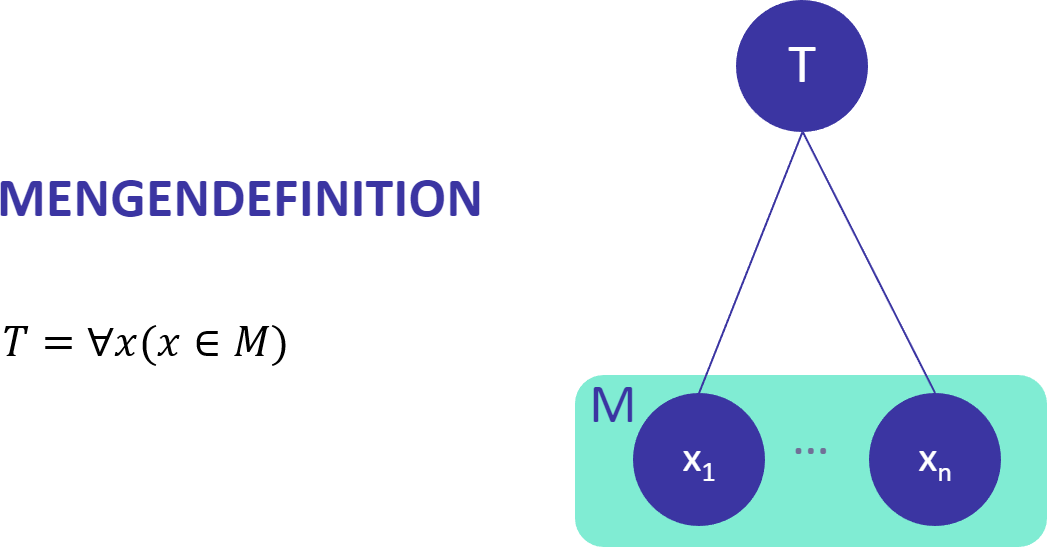
\includegraphics[width=0.5\textwidth]{pictures/therapiedef}
\caption{Aufbau und Beziehungen einer \emph{Therapie}}
\label{therapiedef}
\end{figure}


\subsubsection{Therapiemodul}
Im Rahmen dieses Projekts wird unter \emph{Therapiemodul} das Anwenden  einer Methode zur Behandlung einer Störung mit Krankheitswert oder auch die Aufarbeitung und Überwindung sozialer Konflikte verstanden. Bei diesen Methoden handelt es sich um wissenschaftlich anerkannte psychotherapeutische Verfahren. Den zu behandelnden Störungen mit Krankheitswert wird vorausgesetzt, dass diese als Psychotherapie indiziert sind.

Ein Therapiemodul ist Teil einer Therapie. Das Therapiemodul behandelt ein Aspekt der Therapie.

\paragraph{Definition}
\begin{quote}
Austauschbares, komplexes Element innerhalb eines Gesamtsystems, eines Gerätes o. Ä., das eine geschlossene [Funktions]einheit bildet. \cite{DudenMod70:online}
\end{quote}

\paragraph{Beispiel anhand der aufgestellten Persona}
 \emph{Jonas Vogt} ist 26 Jahre und leidet unter den Spätfolgen eines Burnouts. Seine Psychologische Psychotherapeutin \emph{Dipl.-Psych. Barbara Probst} wendet im Erstgespräch ein Therapiemodul an, welches \emph{Jonas} dabei helfen soll, negative Gedanken zu erkennen und diese für den weiteren Therapieverlauf zu dokumentieren. Ziel des Therapiemoduls ist es, \emph{Jonas} beizubringen, negative Gedanken aufzuschlüsseln und in positive Gedanken umzuformulieren. Im weiteren Verlauf der Therapie wendet \emph{Dipl.-Psych. Barbara Probst} weitere Therapiemodule an um verschiedene Probleme, die zum einen zum Burnout führten und zum anderen aus dem Burnout resultieren, aufzuschlüsseln und \emph{Jonas} den Umgang damit zu erleichtern.

\begin{figure}[h]
\centering
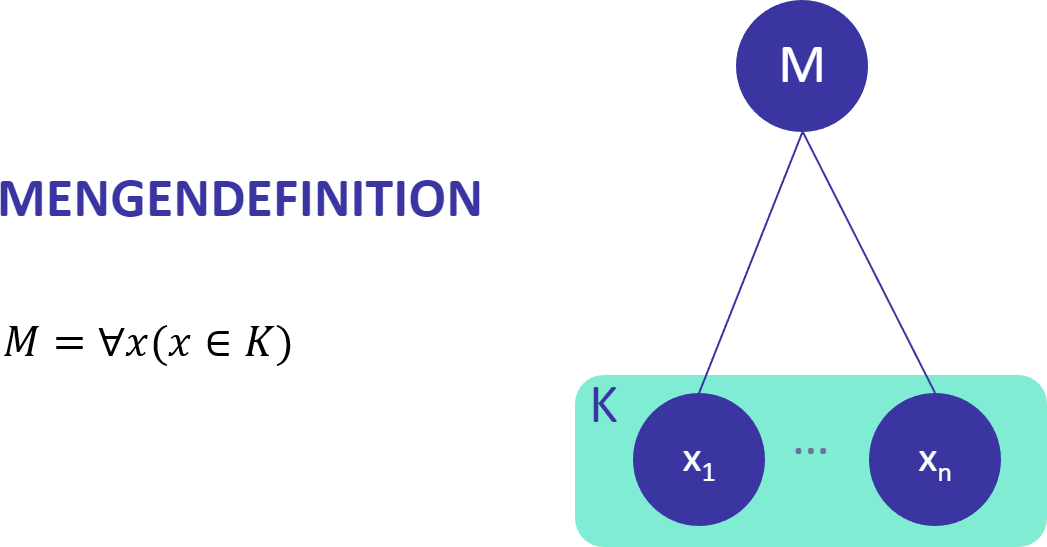
\includegraphics[width=0.5\textwidth]{pictures/moduldef}
\caption{Aufbau und Beziehungen des \emph{Therapiemoduls}}
\label{moduldef}
\end{figure}

\subsubsection{Chatbot-Konversation}
Im Rahmen dieses Projekts wird unter Chatbot-Konversation das Führen  eines Gesprächs mit dem Ziel zur Behandlung/Begleitung einer Störung mit Krankheitswert oder auch die Aufarbeitung und Überwindung sozialer Konflikte verstanden. Die Konversation ist Teil eines Therapiemoduls und kann von Bildern, Video-/Audiomaterial sowie Übungen begleitet werden. Im Kontext des TherapyBuilders wird die Konversation zwischen zwei Parteien geführt: dem Therapeuten oder dem Chatbot und dem Patienten.

\paragraph{Definition}
\begin{quote}
Häufig konventionelles, oberflächliches und unverbindliches Geplauder; Gespräch, das in Gesellschaft nur um der Unterhaltung willen geführt wird. \cite{DudenKon2:online}
\end{quote}

\paragraph{Beispiel anhand der aufgestellten Persona}
\emph{Dipl.-Psych. Barbara Probst} führt pro Therapiesitzung ein Gespräch/eine Konversation mit ihrem Patienten \emph{Jonas Vogt}. In dieser Konversation ermittelt sie \emph{Jonas} aktuellen Zustand, Dinge die in derzeit bewegen und beschäftigen und erklärt ihm den Ursprung seiner Gefühle. Außerdem führt sie mit \emph{Jonas} Übungen durch, die ihm im Alltag helfen können bestimmte wiederkehrende Probleme zu meistern und sein Selbstwert zu stärken.

\begin{figure}[h]
\centering
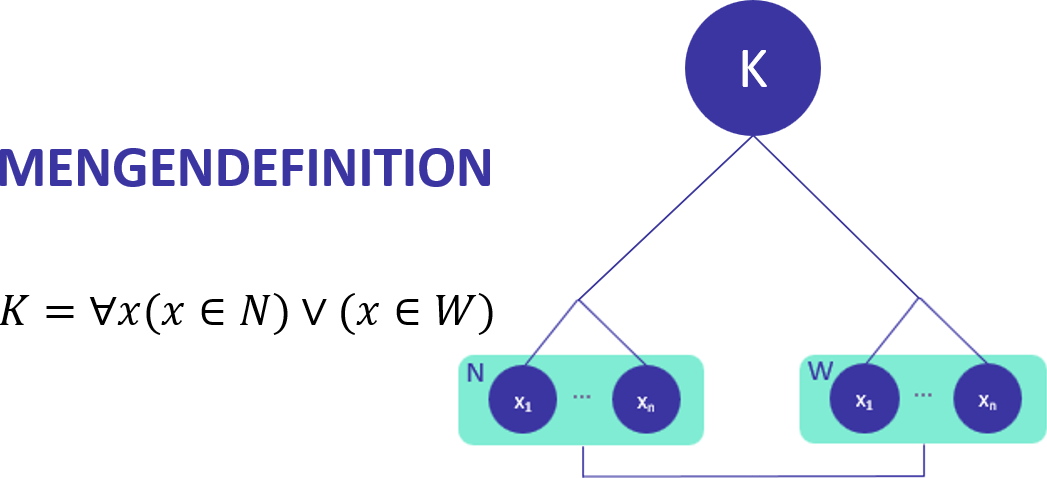
\includegraphics[width=0.5\textwidth]{pictures/konvesationdef}
\caption{Beziehungen der Chatbot-Konversation}
\label{therapiedef}
\end{figure}


\subsubsection{Chatbot-Nachricht}
Im Rahmen dieses Projekts wird unter Chatbot-Nachricht ein Teil einer Therapie-Konversation verstanden. Im Kontext des TherapyBuilders wird zwischen Chatbot und Patient eine Konversation, bestehend aus Nachrichten, aufgebaut. Unterschieden wird innerhalb dieser Konversation zwischen Nachrichten des Patienten und Nachrichten des Chatbots unterschieden. Die Nachrichten des Chatbots können aus folgenden Elementen bestehen: Text, Link, Audio, Video, Bild, Externe Seiteninhalte (Statistiken - Iframe), Telefonnummern. Die Nachrichten des Nutzers können aus folgenden Elementen bestehen: Select One (Quick Reply), Freitext, Likert-Skala, Zahlen (GK, FKZ, Datum, Zeit), Visual-Analog-Skala (VAS).

\paragraph{Definition}
\begin{quote}
Mitteilung, die jemandem in Bezug auf jemanden oder etwas [für ihn persönlich] Wichtiges die Kenntnis des neuesten Sachverhalts vermittelt. \cite{DudenNac9:online}
\end{quote}

\paragraph{Beispiel anhand der aufgestellten Persona}
\emph{Jonas Vogt} erhielt im Erstgespräch mit seiner Psychologischen Psychotherapeutin \emph{Dipl.-Psych. Barbara Probst} die Empfehlung die Anwendung „TherapyBuilder“ auf dessen Smartphone zu installieren. \emph{Jonas} soll diesen zunächst bis zum ersten Behandlungstermin nutzen. Frau \emph{Dipl.-Psych. Barbara Probst} legt für \emph{Jonas} fest, welche Therapiemodule bis dahin für \emph{Jonas} zur Verfügung stehen. \emph{Jonas} kommuniziert täglich mit dem Chatbot des TherapyBuilders. Die Art der Nachrichten des Chatbots sowie des Anwenders \emph{Jonas} wurden bereits als Therapiemodul konfiguriert und festgelegt. Der Chatbot kommuniziert mit \emph{Jonas} via Text, Link, Audio, Video, Bild, Externe Seiteninhalte (Statistiken - Iframe), Telefonnummern. \emph{Jonas} selbst nutzt Eingabeformate wie Select One (Quick Reply), Freitext, Likert-Skala, Zahlen (GK, FKZ, Datum, Zeit), Visual-Analog-Skala (VAS). Wann er welche als Nachricht an den Chatbot versendet, ist innerhalb des Therapiemoduls geregelt.

\begin{figure}[h]
\centering
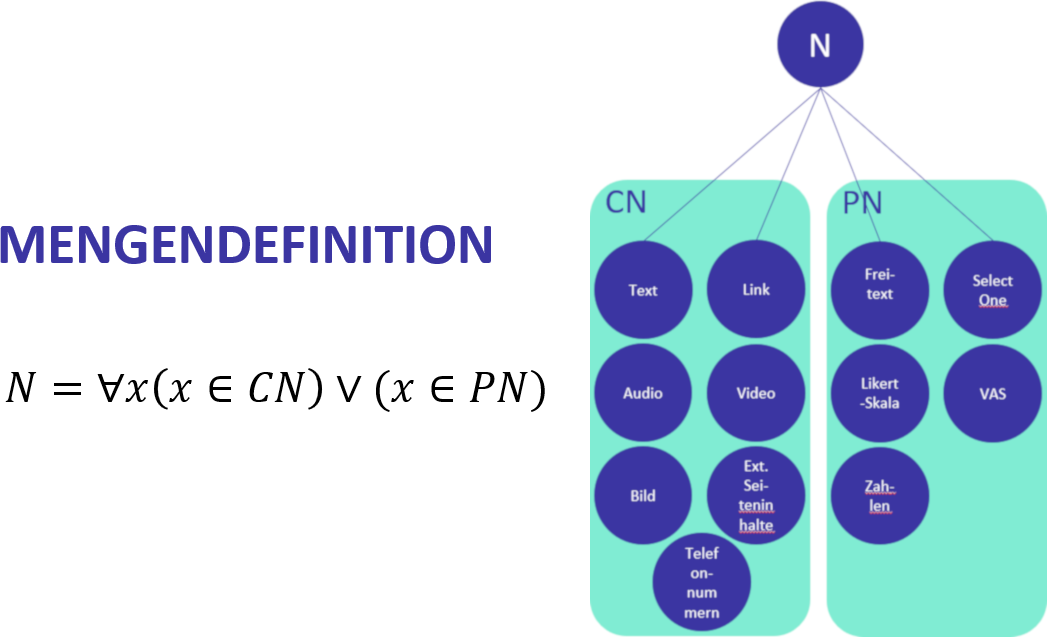
\includegraphics[width=0.5\textwidth]{pictures/nachrichtdef}
\caption{Beziehungen der Chatbot-Nachrichten}
\label{therapiedef}
\end{figure}

\subsubsection{Werkzeugkasten}
Im Rahmen dieses Projekts wird unter Werkzeugkasten ein Teil eines Therapie-Moduls verstanden welches Techniken (=Werkzeuge) sammelt, die jederzeit wiederholt ausgeführt werden können. Diese sollen den Nutzer unterstützen bestimmte (Denk- oder Verhaltens-) Muster zu erkennen und diese aufzulösen. Dies geschieht unter Zuhilfenahme bestimmter Techniken. In diesem Teil wird der Nutzer angeleitet eine bestimmte Vorgehensweise durchzuführen, um diese Techniken auf bestimmte Denk- oder Verhaltensmuster anzuwenden. Der Nutzer kann diese Techniken jederzeit im Werkzeugkasten als Werkzeug aufrufen wenn benötigt.

\paragraph{Definition}
\begin{quote}
Kasten zur Aufbewahrung von Werkzeug. \cite{DudenWer23:online}
\end{quote}

\paragraph{Beispiel anhand der aufgestellten Persona}
\emph{Dipl.-Psych. Barbara Probst} rät \emph{Jonas Vogt} bis zum ersten Behandlungstermin die Therapiemodule durchzuführen, die sie in \emph{Jonas} Therapieplan ablegt. Sie unterrichtet \emph{Jonas}, dass diese Hilfreiche Werkzeuge für bestimmte Denk- und Verhaltensmuster enthalten. Diese müssen durch einen Fortschritt im Therapiemodul freigeschaltet und können ab diesem Zeitpunkt jederzeit von \emph{Jonas} aufgerufen werden. Das erste Werkzeug welches \emph{Jonas} aktiviert, ist das Werkzeug für das Auflösen negativer Gedanken. Sobald \emph{Jonas} negative Gedanken hat, führt er dieses Werkzeug erneut aus um die negativen Gedanken aufzulösen.

\begin{figure}[h]
\centering
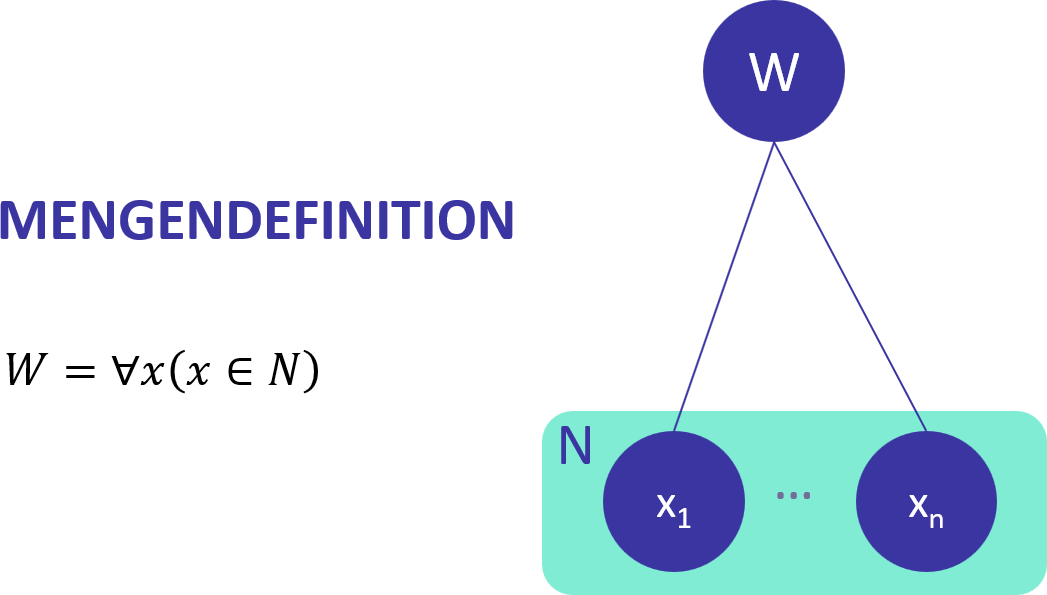
\includegraphics[width=0.5\textwidth]{pictures/toolboxdef}
\caption{Beziehungen der Mengen}
\label{therapiedef}
\end{figure}



\subsection{Konzepte}

